\documentclass[10pt,a4paper]{article}
\usepackage[utf8]{inputenc}
\usepackage[english]{babel}
\usepackage[activate={true,nocompatibility},final,tracking=true,kerning=true,spacing=true]{microtype}
\usepackage[plainpages=false,pdfpagelabels,unicode]{hyperref}
\usepackage{fullpage}
\usepackage{graphicx}
\usepackage{fancyhdr}
\usepackage{comment}
\usepackage{occi}
\usepackage{tabularx}
\setlength{\headheight}{13pt}
\pagestyle{fancy}

% default sans-serif
\renewcommand{\familydefault}{\sfdefault}

% no lines for headers and footers
\renewcommand{\headrulewidth}{0pt}
\renewcommand{\footrulewidth}{0pt}

% header
\fancyhf{}
\lhead{GFD-R}
\rhead{\today}

% footer
\lfoot{occi-wg@ogf.org}
\rfoot{\thepage}

% paragraphs need some space...
\setlength{\parindent}{0pt}
\setlength{\parskip}{1ex plus 0.5ex minus 0.2ex}

% some space between header and text...
\headsep 13pt

\setcounter{secnumdepth}{4}

\begin{document}

% header on first page is different
\thispagestyle{empty}

Draft \hfill  {Ralf Nyrén, Independent}\\
OCCI-WG \hfill  Andy Edmonds, ICCLab, ZHAW
\rightline {Alexander Papaspyrou, Adesso}
\rightline {Thijs Metsch, Intel}
\rightline {Boris Parák, CESNET}
\rightline {April 7, 2011}\\
\rightline {Update: \today}

\vspace*{0.5in}

\begin{Large}
\textbf{Open Cloud Computing Interface -- Core}
\end{Large}

\vspace*{0.5in}

\underline{Status of this Document}

This document provides information to the community regarding the
specification of the Open Cloud Computing Interface. Distribution is
unlimited.


\underline{Copyright Notice}

Copyright \copyright{}~Open Grid Forum (2009--2015). All Rights Reserved.

\underline{Trademarks}

OCCI is a trademark of the Open Grid Forum.

\underline{Abstract}

This document, part of a document series, produced by the OCCI working
group within the Open Grid Forum (OGF), provides a high-level
definition of a Protocol and API. The document is based upon
previously gathered requirements and focuses on the scope of important
capabilities required to support modern service offerings.


\newpage
\tableofcontents
\newpage

\section{Introduction}
%!TEX root = nml-base.tex

\section{Introduction}%
\label{sec:introduction}

This document describes the base schema of the Network Markup Language (NML).
Section~\ref{sub:classes} defines the NML classes and their attributes and parameters.
Section~\ref{sub:relations} describes the relations defined between NML classes.

An NML network description can be expressed in XML\cite{xml}, and RDF/XML\cite{rdfxml} syntax.
Section~\ref{s:xmlschema} describes the XSD schema for the XML syntax.
Section~\ref{s:owlschema} describes the OWL 2 schema for the RDF/XML syntax.

These basic classes defined in this document may be extended, or sub-classed, 
to represent technology specific classes.

Section~\ref{s:examples} provides example use cases. This section is informative. 
Only sections~\ref{s:schema}, \ref{s:identifiers}, \ref{s:syntax}, and appendices \ref{s:xmlschema} and \ref{s:owlschema} are normative and considered 
part of the recommendation.

Appendix~\ref{s:g800terms} is informative and explains the relation between terms defined in this document and those defined in the ITU-T G.800 recommendation~\cite{g800}.

\subsection{Context}
\label{sec:context}

The Network Markup Language (NML) has been defined in the context of research and 
education networks to describe so-called hybrid network topologies. The NML is defined
as an abstract and generic model, so it can be applied for other network topologies as well.
See \cite{gfd.165} for an detailed overview including prior work.

\subsection{Scope}
\label{sec:scope}

The Network Markup Language is designed to create a functional description of 
multi-layer networks and multi-domain networks. An example of a multi-layered 
network can be a virtualised network, but also using different technologies. 
The multi-domain network descriptions can include aggregated or abstracted network topologies.
NML can not only describe a primarily static network topology, but also its potential capabilities (services) 
and its configuration.

NML is aimed at logical connection-oriented network topologies, more precisely topologies
where switching is performed on a label associated with a flow, such as a VLAN, wavelength or time slot. 
NML can also be used to describe physical networks or packet-oriented networks, 
although the current base schema does not contain classes or properties 
to explicitly deal with signal degradation, or complex routing tables.

NML only attempts to describe the data plane of a computer network, not the control 
plane. It does contain extension mechanism to easily tie it with network provisioning 
standards and with network monitoring standards.

Finally, this document omits a definition for the terms \emph{Network} or \emph{capacity}. 
This has been a conscious choice. The term \emph{Network} has become 
so widely used for so many diverse meanings that it is impossible to create a 
definition that everyone can agree on, while still expressing something useful.
See \emph{Topology} for the concept of a network domain and a \emph{Link} with multiple 
sources and sinks for the concept of a local area network.
The term \emph{capacity} is used by different technologies in such a different 
way (e.g.\ including or excluding the header and footer overhead) that it is better 
to let technology-specific extensions make an explicit definition.

\subsection{Notational Conventions}%
\label{sec:rfc2119}

The keywords “\MUST{}”, “\MUSTNOT{}”, “\REQUIRED{}”, “\SHALL{}”, “\SHALLNOT{}”, 
“\SHOULD{}”, “\SHOULDNOT{}”, “\RECOMMENDED{}”, “\MAY{}”,  and “\OPTIONAL{}” are 
to be interpreted as described in \cite{rfc2119}.
% except that the words do not appear in uppercase. 

This schema defines classes, attributes, relations, parameters and logic.
Objects are instances of classes, and the type of an object is a class.

Names of classes are capitalised and written in italics (e.g.\ the \emph{Node} class).
Names of relations are written in camel case and in italics (e.g.\ the \emph{hasNode} relation).
Names of identifiers and string literals are written in monspaces font (e.g. \texttt{Port\_X:in}).

Diagrams in this document follow the diagrammatic conventions of UML class diagrams.
\begin{itemize}
\item A subclass-superclass relationship is represented by a line with hollow triangle shape pointing to the superclass.
\item A whole-part relationship is represented by a line with a hollow diamond shape pointing to the whole (group).
\item A entity-relationship is represented by a line, optionally with numbers at each end indicating the cardinality of the relation. A named entity-relationship has a verb next to the line, and a filled triangle pointing to the object of the verb. (e.g. the entitity-relationship
\nmlrelation{BidirectionalPort}{*}{hasPort}{2}{Port} is named \emph{hasPort}, and each \emph{BidirectionalPort} is related to exactly 2 \emph{Port}s, and each \emph{Port} may be associated with zero, one or more \emph{BidirectionalPort}s.)
\end{itemize}



\section{Notational Conventions}
All these parts and the information within are mandatory for
implementors (unless otherwise specified). The key words "MUST", "MUST
NOT", "REQUIRED", "SHALL", "SHALL NOT", "SHOULD", "SHOULD NOT",
"RECOMMENDED", "MAY", and "OPTIONAL" in this document are to be
interpreted as described in RFC 2119 \cite{rfc2119}.


\section{Terms and definitions}
Section \ref{sec:glossary} provides a glossary of all terms and
definitions with a specific meaning to the OCCI specification
suite. However, for reader convenience, a sub-set of the glossary is
provided here as well. The following terminology has specific meaning
in the OCCI context:

\begin{description}
  \item[capabilities] In the context of \hl{Entity} sub-types
    {\bf  capabilities} refer to the \hl{Attribute}s and \hl{Action}s
    exposed by an {\bf entity instance}.

  \item[entity instance] An instance of a sub-type of
    \hl{Entity} but not an instance of the \hl{Entity} type itself.
    The OCCI model defines two sub-types of \hl{Entity}:
    the \hl{Resource} type and the \hl{Link} type.  However, the term
    {\bf entity instance} is defined to include any instance of a
    {\em sub-type} of \hl{Resource} or \hl{Link} as well.

  \item[mix-in] An instance of the \hl{Mixin} type associated with an
    {\bf entity instance}. The \textbf{mix-in} concept as used by OCCI
    {\em only} applies to instances, never to \hl{Entity} types.
    See section~\ref{sec:mixin}.

  \item[model attribute] An attribute of the Core Model.

  \item[OCCI base type(s)] The OCCI base types are \hl{Entity},
    \hl{Resource} and \hl{Link}.
    See section~\ref{sec:base_types}.

  \item[template] A mechanism to provide default values for an {\bf entity
    instance}. See section~\ref{sec:template}.

  \item[type] A {\bf type} refers to one of those defined by the OCCI
    Core Model.  The OCCI Core Model types are \hl{Category},
    \hl{Attribute},
    \hl{Kind}, \hl{Mixin}, \hl{Action}, \hl{Entity}, \hl{Resource} and
    \hl{Link}.

  \item[concrete type/sub-type] A \textbf{concrete type} or \textbf{sub-type} is a \textbf{type} that can
    be instantiated.
\end{description}

\section{OCCI Core}
The Open Cloud Computing Interface is a boundary protocol and API that
acts as a service front-end to a provider's internal management
framework. Figure~\ref{fig:placement} shows OCCI's place in a
provider's architecture.

\begin{figure}[h]
  \centering
  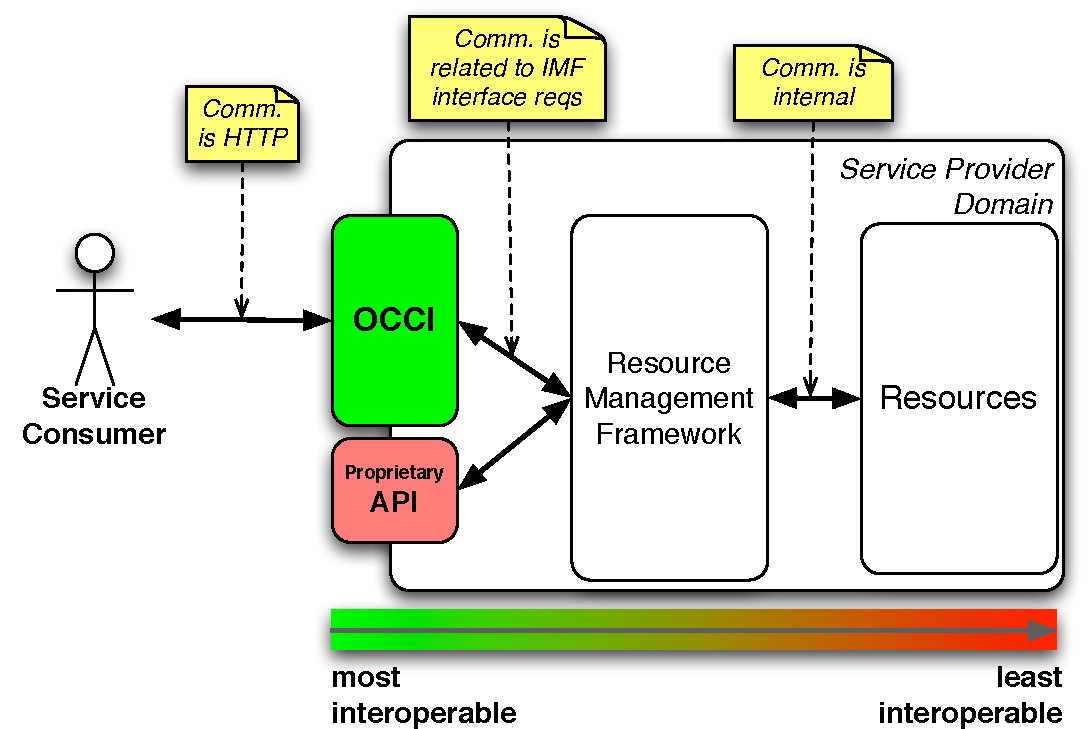
\includegraphics[scale=0.5]{figs/occi-intro.pdf}
  \caption{OCCI's place in a provider's architecture.}
  \label{fig:placement}
\end{figure}

Service consumers can be both end-users and other system
instances. OCCI is suitable for both cases. The key feature is that
OCCI can be used as a management API for all kinds of resources while
at the same time maintaining a high level of interoperability.

This document, the OCCI Core specification, defines the OCCI Core
Model. This model is the core of the specification suite. Renderings
(including associated behaviors) can interact with it and extensions
can expand it. In itself, the core model is only useful
for a very limited set of use cases. However, it provides the basis
for renderings and extensions to build upon.

\section{OCCI Core Model}
The OCCI Core Model defines a representation of instance types which
can be manipulated through an OCCI protocol and rendering implementations.
It is an abstraction of real-world resources, including the means to identify,
classify, associate and extend those resources.

A fundamental feature of the OCCI Core Model is that it can be
extended in such a way that any extension will be discoverable and
visible to an OCCI client at run-time. An OCCI client can connect to
an OCCI implementation using an extended OCCI Core Model, without
knowing anything in advance, and still be able to discover and
understand, at run-time, the various instance types
supported by that implementation.
For example, a
web-based OCCI client could easily be reused as the management tool
for a wide variety of services.

The OCCI Core Model can be extended through inheritance but also
using a mixin-like concept.

\begin{quote}
  Mixins first appeared in the Symbolics' object-oriented
  Flavors~\cite{Moon:1986:flavors} system (developed by Howard
  Cannon), which was an approach to object-orientation used in Lisp
  Machine Lisp.%
  \footnote{http://en.wikipedia.org/wiki/Mixin.}
\end{quote}

The mix-in model only applies at the instance level, i.e., the ``object
level'', and thereby differs from the more common uses of the mix-in
concept. A mix-in in OCCI can never be applied to a type, only to an
instance.

\subsection{Overview}

The UML class diagram shown in figure~\ref{fig:occi_model} gives an
overview of the OCCI Core Model. It must be noted that the UML diagram
in itself is not a complete definition of the model. The diagram is
merely provided as an overview to help understanding the model.

\begin{figure}[!h]
  {\centering \resizebox*{0.9\columnwidth}{!}{%\rotatebox{270}
      {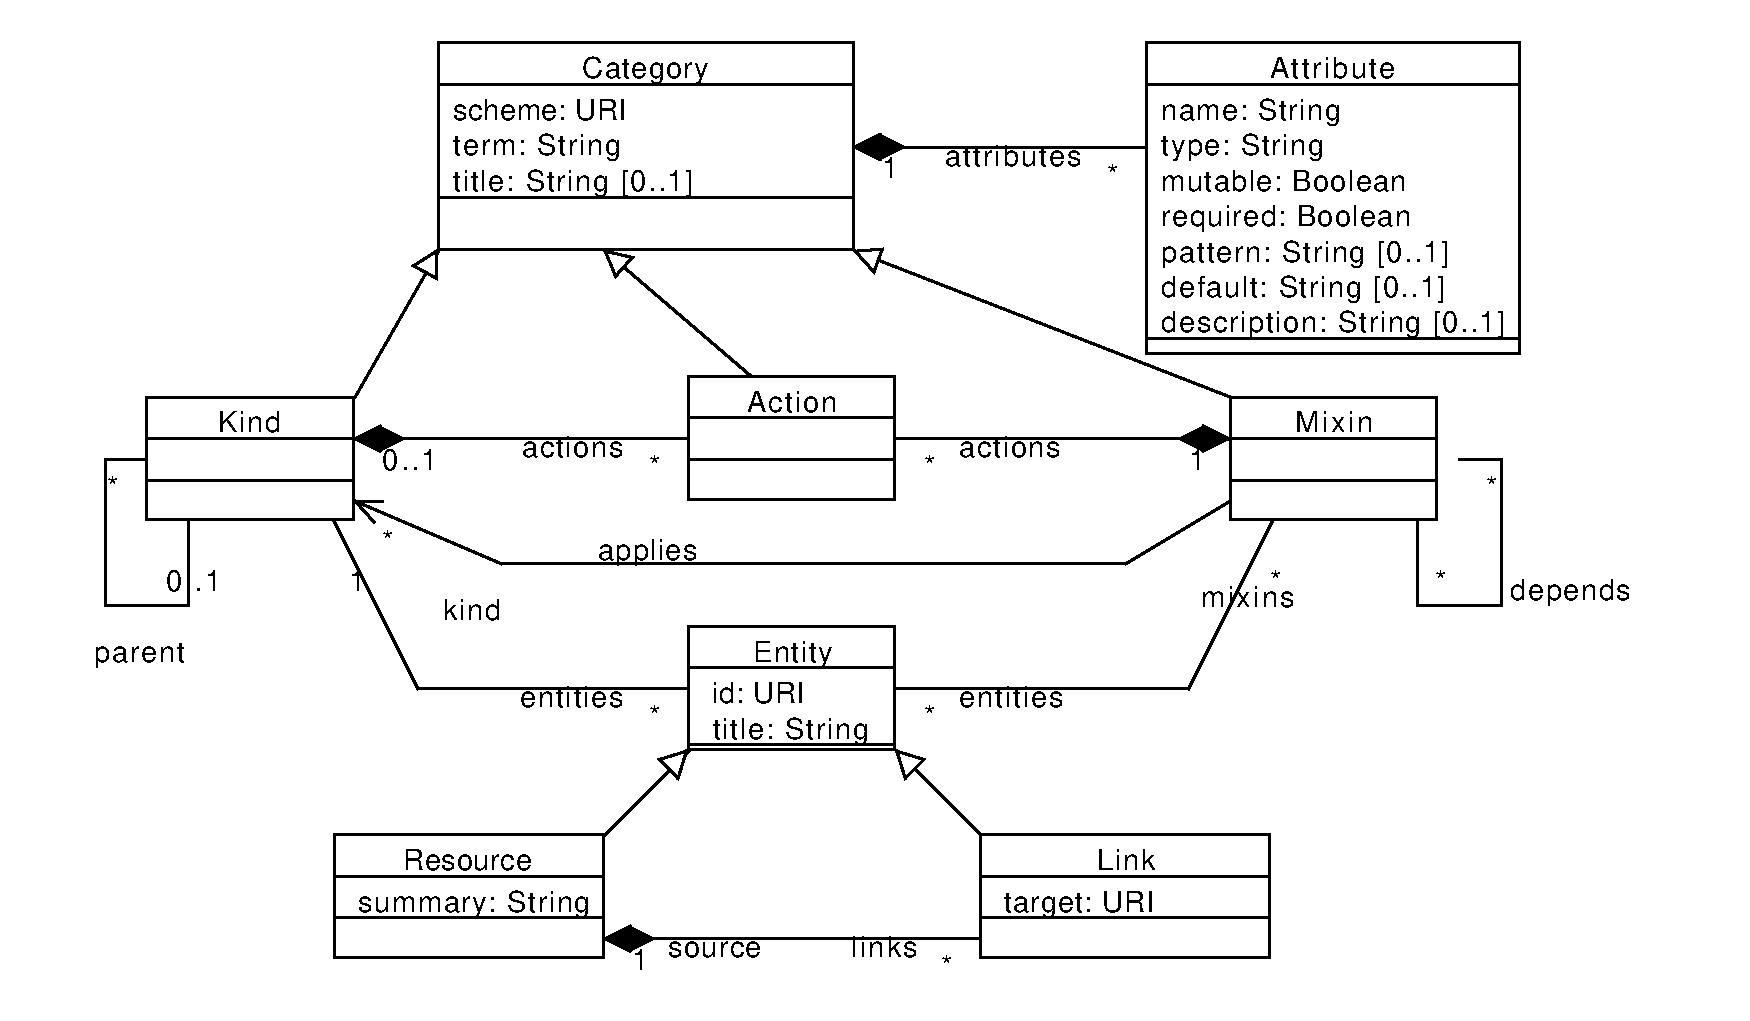
\includegraphics{figs/core_model.pdf}}} \par}
  \caption{UML class diagram of the OCCI Core Model. The diagram
    provides an overview of the OCCI Core Model but is not a
    standalone definition thereof.}
  \label{fig:occi_model}
\end{figure}

The heart of the OCCI Core Model is the \hl{Resource} type. Any
resource exposed through OCCI is a \hl{Resource} or a sub-type
thereof.  A resource can be, e.g., a virtual machine, a job in a job
submission system, a user, etc.

The \hl{Resource} type contains a number of common attributes that
\hl{Resource} sub-types inherit. The \hl{Resource} type is
complemented by the \hl{Link} type which associates one \hl{Resource}
instance with another.
%
The \hl{Link} type contains a number of common attributes that
\hl{Link} sub-types inherit.

\hl{Entity} is an abstract type, which both \hl{Resource} and \hl{Link}
inherit.  Each sub-type of \hl{Entity} is identified by a unique
\hl{Kind} instance.

The \hl{Kind} type is the core of the type classification system built
into the OCCI Core Model. \hl{Kind} is a specialization of
\hl{Category} and introduces additional capabilities in terms
of \hl{Action}s.  An \hl{Action} identifies an invocable operation
applicable to an entity instance.

\hl{Attribute}s describe the name and properties of attributes found in
\hl{Entity} and its sub-types.

The last type defined by the OCCI Core Model is the \hl{Mixin}
type. An instance of \hl{Mixin} can be associated with an entity
instance to mix-in additional capabilities at run-time.

For compliance with OCCI Core, all of the types defined in the OCCI
Core Model MUST be implemented.  The following sections of the
specification contain the formal definition of the OCCI Core Model.

\subsection{Mutability}
\label{sec:mutability}
\hl{Attribute}s of an OCCI Core Model type instance are either client
mutable or client immutable. If an attribute is noted to be mutable
this MUST be interpreted that a client can create an instance that is
parametrized by the attribute. Likewise, if an attribute is mutable, a
client can update that instance's mutable attribute value and the
server side MUST support this. If an attribute is marked as immutable,
it indicates that the server side implementation MUST manage these
exclusively. Immutable attributes MUST NOT be modifiable by clients
under any circumstance.

\subsection{Classification and Identification}
\label{sec:classification}
The OCCI Core Model provides a built-in type classification system
allowing for safe extension towards domain-specific usage
(e.g., infrastructure). This system is the OCCI type system and offers
the means to be easily and transparently (i.e., no format translation
required) exposed over either a text- or binary-based protocol.

The classification system can be summarized with the following key
features:

\begin{itemize}
  \item Each OCCI base type and extension thereof is assigned a unique
    type identifier (a \hl{Kind} instance), which allows for dynamic
    discovery of available types. All \hl{Entity} sub-types, including
    core model extensions, are assigned a unique \hl{Kind} instance.

  \item The inheritance structure of \hl{Entity}, \hl{Resource} and
    \hl{Link} is client-discoverable. This also applies to any
    sub-type of \hl{Resource} and \hl{Link} and therefore an OCCI
    client can discover the type inheritance structure used by a
    particular OCCI implementation. The discovery of the inheritance
    structure is made possible through the relationship of \hl{Kind}
    instances.

  \item The classification system allows \hl{Mixin} instances to be
    associated to \hl{Entity} instances in order to assign additional
    capabilities in terms of \hl{Attribute}s and \hl{Action}s at
    run-time.

  \item Tagging of \hl{Entity} instances is supported through the
    association of \hl{Mixin} instances. A tag is simply a \hl{Mixin}
    instance, which defines no additional capabilities.

  \item A collection of associated \hl{Entity} instances is implicitly
    defined for each \hl{Kind} and \hl{Mixin} instance. That is, all
    \hl{Entity} instances associated with a particular \hl{Kind} or
    \hl{Mixin} instance form a collection.
\end{itemize}

\subsubsection{Category}
\label{sec:category}
The \hl{Category} type is the basis of the type identification
mechanism used by the OCCI classification system. It MUST be
implemented.
There are no instances of the \hl{Category} type itself in the OCCI Core Model.
The \hl{Category} type is only used through its sub-types \hl{Kind}, \hl{Mixin}
and \hl{Action}.
%
Table~\ref{tbl:category} defines the model attributes the \hl{Category} type
MUST implement to be compliant.

\mytablefloat{
  \label{tbl:category}Model attributes defined for the \hl{Category} type.}{
  \begin{tabularx}{\textwidth}{lllllX}
    \toprule
    Model attribute   & Type    & Value Multiplicity  & Required  & Client Mutability   & Description \\
    \colrule
    term              & String  & 1                   & Yes       & Immutable           & Unique identifier of the \hl{Category} instance within the categorization scheme. \\
    scheme            & URI     & 1                   & Yes       & Immutable           & The categorization scheme. \\
    title             & String  & 0..1                & --        & Immutable           & The display name of an instance. \\
    \botrule
  \end{tabularx}
}

A \hl{Category} instance is uniquely identified by concatenating the
categorization scheme with the category term,
e.g.,~\textit{http://example.com/category/scheme\#term}.  This is done
to enable discovery of \hl{Category} definitions in text-based
renderings such as the OCCI Text Rendering~\cite{occi:text}. All renderings
MUST make use of and understand concatenated unique type identifiers of \hl{Category}
instances.
%
Sub-types of \hl{Category} such as \hl{Kind}, \hl{Mixin} and \hl{Action} inherit
this property.

The categorization schemes defined in the OCCI specification all use
the \textit{http://schemas.ogf.org/occi/} base URL. This base URL is
reserved for OCCI an MUST NOT be used by service provider extensions.

A \hl{Category} instance%
\footnote{Also applies to \hl{Kind}, \hl{Mixin} and \hl{Action} instances.}
has zero or more associated \hl{Attribute} instances.
Each \hl{Attribute}, see section~\ref{sec:attribute},
describes the name and properties of a single attribute.


\subsubsection{Attribute}
\label{sec:attribute}

The \hl{Attribute} type has a composite relationship to \hl{Category} and
defines the name and properties of client readable \hl{Attribute}s.
%
Table~\ref{tbl:attribute} defines the model attributes the \hl{Attribute} type
MUST implement to be compliant.

\mytablefloat{
  \label{tbl:attribute}Model attributes defined for the \hl{Attribute} type.}{
  \begin{tabularx}{\textwidth}{lp{18mm}lllX}
    \toprule
    Model attribute & Type                        & Value Multiplicity  & Required  & Client Mutability   & Description \\
    \colrule
    name            & String                      & 1                   & Yes       & Immutable           & Attribute name. \\
    type            & Enum \{Object, List, Hash\} & 1                   & Yes       & Immutable           & Attribute type. \\
    mutable         & Boolean                     & 1                   & Yes       & Immutable           & Attribute mutability. \\
    required        & Boolean                     & 1                   & Yes       & Immutable           & Whether the Attribute must be supplied by the client at instance creation-time. \\
    pattern         & Object                      & 0..1                & --        & Immutable           & Attribute pattern expressed in a rendering-specific way. \\
    default         & \{Object, List, Hash\}      & 0..1                & --        & Immutable           & Attribute default value. \\
    description     & String                      & 0..1                & --        & Immutable           & A description of the Attribute. \\
    \botrule
  \end{tabularx}
}

An Attribute name MUST be defined by \hl{Attribute}.{\tt name}. The
Attribute namespace is flat and the ``\texttt{occi.}''~prefix is reserved
for the OCCI specification.
Domain-specific Attribute names MUST NOT contain the
``\texttt{occi.}''~prefix, instead they SHOULD use a prefix consisting of the
provider's reverse domain name. E.g.,~``\texttt{com.example.}''.

An \hl{Attribute} MAY specify the following properties in addition to the
Attribute name. Attribute properties are OPTIONAL but MUST be client
discoverable if used.
\begin{description}
\item[type] The type of the \hl{Attribute}. The types supported are ``Object'', ``List'' and ``Hash''.

\item[mutable] Whether an OCCI client can change the Attribute value. See
  section~\ref{sec:mutability}.

\item[required] If an \hl{Attribute} is ``required'' a client MUST specify a
  value at instance creation-time.

\item[pattern] MAY be specified in a rendering-specific format, places additional restrictions on acceptable attribute values. Detailed
  information is provided in every OCCI rendering document.

\item[default] The default value given to an \hl{Attribute} if the client does
  not specify a value at instance creation time.  The {\em default} property is used to implement templates, see section~\ref{sec:template}.

\item[description] A summarizing description of the \hl{Attribute} to
  complement the attribute name. For example, an interactive OCCI client may
  use the description property when presenting the content of an entity
  instance.
\end{description}


\subsubsection{Kind}
\label{sec:kind}

The \hl{Kind} type, together with the \hl{Mixin} type, defines the
classification system of the OCCI Core Model. It MUST be
implemented. The \hl{Kind} type represents the type identification
mechanism for all \hl{Entity} types present in the model.
%
Sub-types MUST NOT be derived from the \hl{Kind} type.

A unique \hl{Kind} {\em instance} MUST be assigned to each and every
\hl{Entity} sub-type defined in an OCCI implementation.

Every instance of \hl{Kind} represents a unique type identifier for a
particular sub-{\em type} of \hl{Entity}.  Consequently, when an \hl{Entity}
sub-type is instantiated the entity instance MUST be associated with
its type identifier, i.e.,~the \hl{Kind} instance.  An entity instance
MUST remain associated with its \hl{Kind} instance throughout its
lifetime.
%
For example an instance of \hl{Resource} MUST always be associated
with the \hl{Kind} instance which identifies the \hl{Resource} {\em type}.

In the initial instantiation of the OCCI Core Model, with no core
model extensions, three instances of \hl{Kind} will be present: one
for \hl{Entity}, another for \hl{Resource} and the last one for
\hl{Link}.

\mytablefloat{
  \label{tbl:kind}Model attributes defined for the \hl{Kind} type.}{
  \begin{tabularx}{\textwidth}{lllllX}
    \toprule
    Model attribute & Type                  & Value Multiplicity  & Required  & Client Mutability     & Description \\
    \colrule
    actions         & List of \hl{Action}   & 0..*                & --        & Immutable             & List of \hl{Action} instances defined by the \hl{Kind} instance. \\
    parent          & \hl{Kind}             & 0..1                & --        & Immutable             & Another \hl{Kind} instance which this \hl{Kind} has an inheritance relationship with. \\
    entities        & List of \hl{Entity}   & 0..*                & --        & Immutable             & List of \hl{Entity} instances. Instances of the particular \hl{Entity} sub-type which is uniquely identified by this \hl{Kind} instance. \\
    \botrule
  \end{tabularx}
}

The \hl{Kind} type inherits the \hl{Category} type. To be compliant
the \hl{Kind} type MUST implement the model attributes defined in
table~\ref{tbl:kind} and the inherited model attributes defined in
table~\ref{tbl:category}. The following rules apply to all instances
of the \hl{Kind} type:
%
\begin{itemize}
  \item A unique \hl{Kind} instance MUST be assigned to each and every
    sub-type of \hl{Entity}, including \hl{Entity} itself.

  \item A \hl{Kind} instance MUST expose the discoverable attributes defined for
    the \hl{Entity} sub-type it identifies.

  \item A \hl{Kind} instance MUST expose the \hl{Action}s defined for
    its \hl{Entity} sub-type.

  \item A \hl{Kind} instance MUST have the \hl{Kind} instance of \hl{Entity}%
    \footnote{\textit{http://schemas.ogf.org/occi/core\#entity}}
    as its parent.

  \item If type {\bf B} inherits type {\bf A}, where {\bf A} is a
    sub-type of \hl{Entity}, the \hl{Kind} instance of {\bf B} MUST
    have its {\tt parent} attribute set to the \hl{Kind} instance of {\bf A}.
    See Kind Relationships below.
\end{itemize}

\paragraph*{Kind Relationships}
A relationship between \hl{Kind} instances is defined by the ``{\tt parent}'' attribute. This implies a setup of a hierarchy where the capabilities of the parent MUST be inherited by the child \hl{Kind} instance.

\begin{figure}[!h]
  {\centering \resizebox*{0.9\columnwidth}{!}{\rotatebox{0}
      {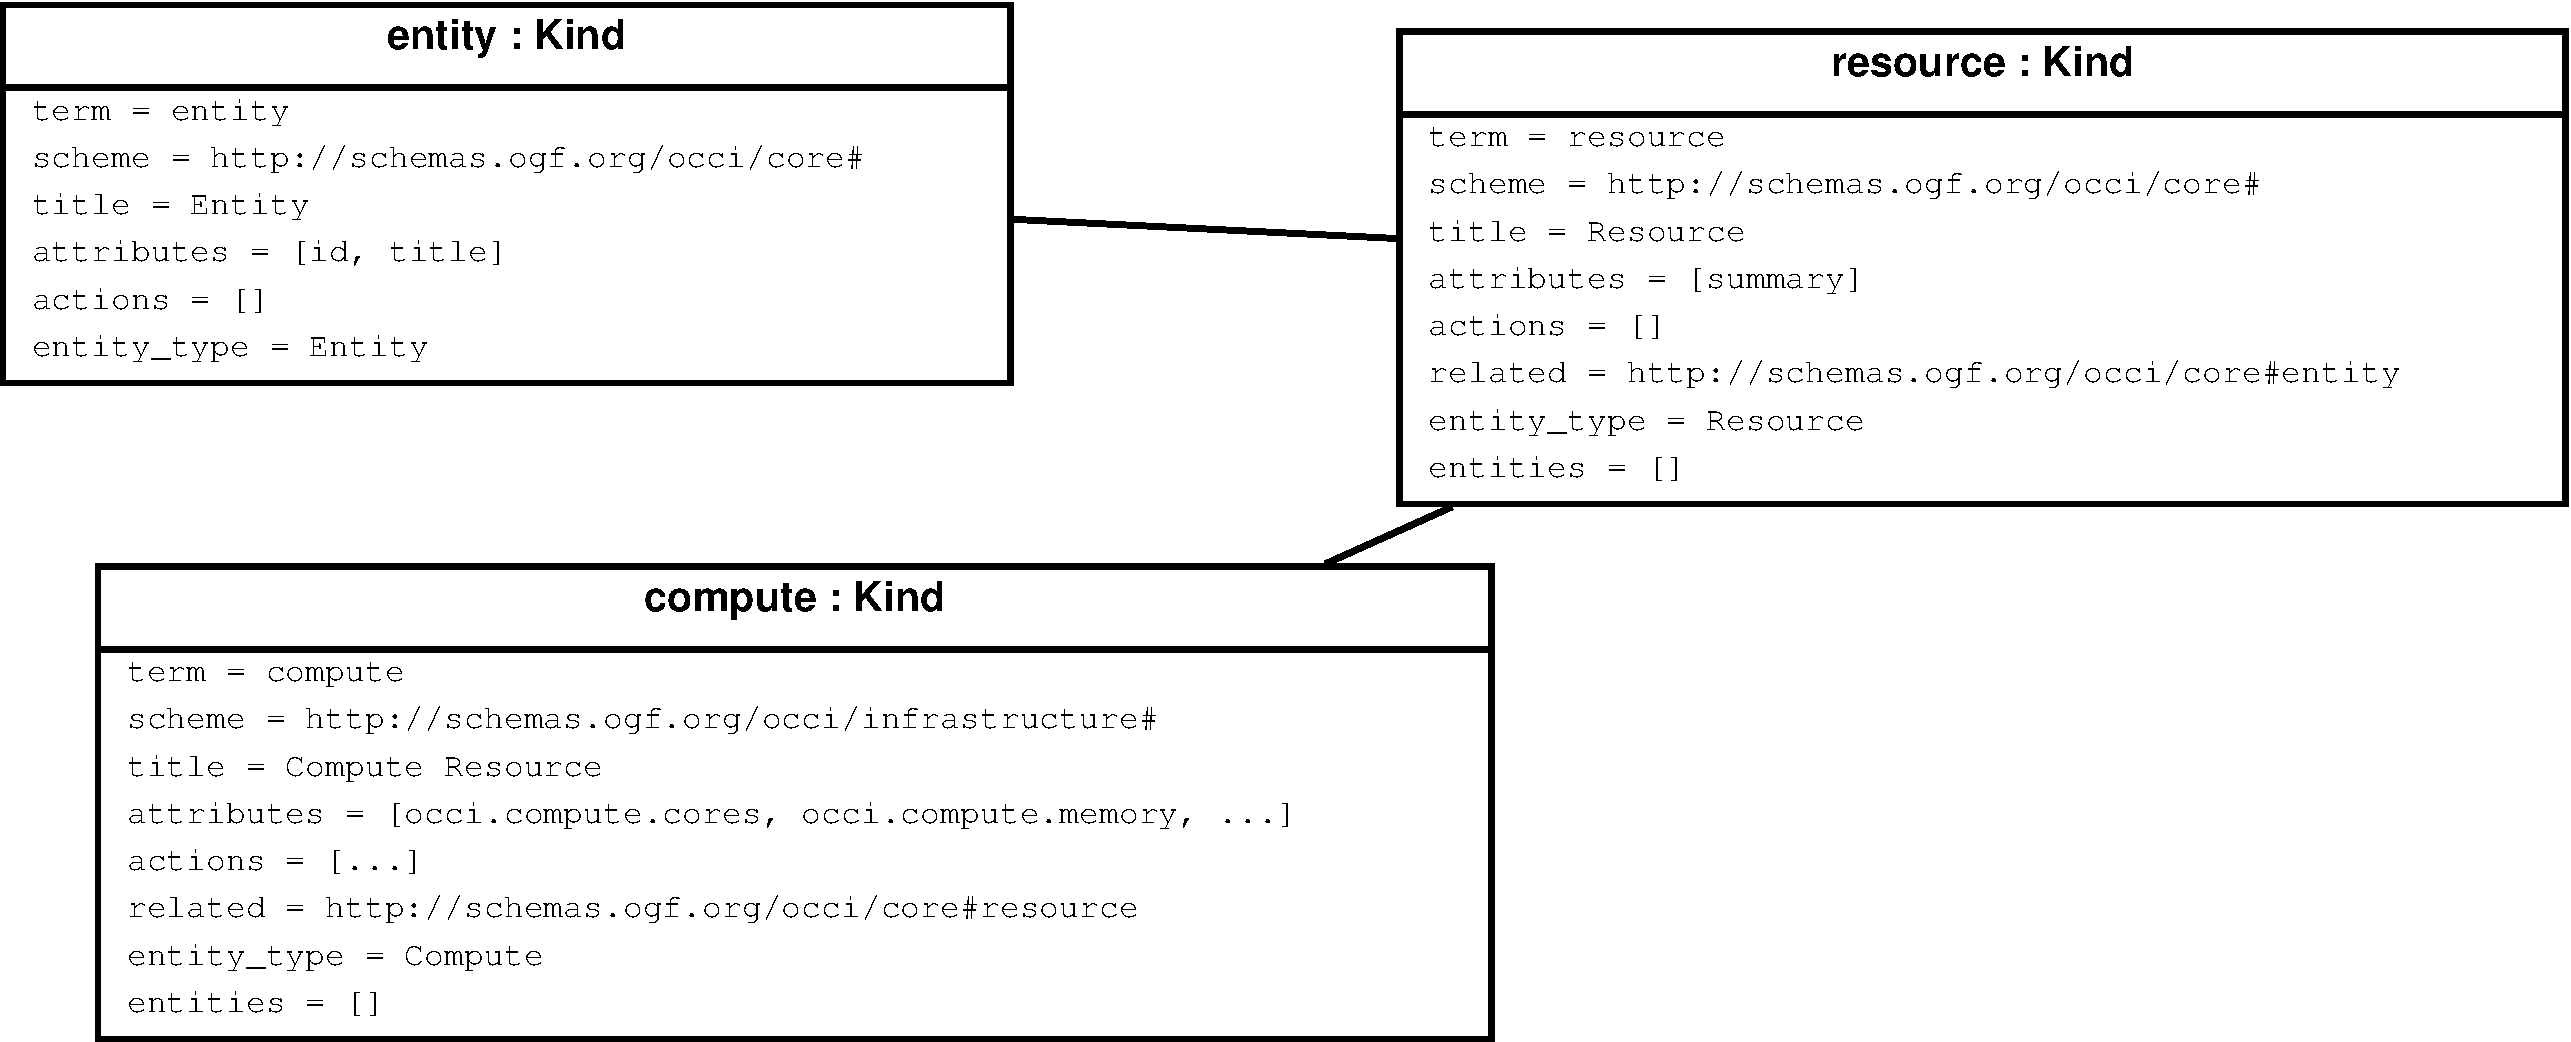
\includegraphics{figs/kind_relationships.pdf}}} \par}
  \caption{Object diagram illustrating the \hl{Kind} instances
    involved for the \hl{Entity}, \hl{Resource} and \hl{Compute}
    types. The \hl{Compute} type is an extension to the OCCI Core
    Model defined in the OCCI Infrastructure
    document~\cite{occi:infrastructure}.}
  \label{fig:kind_relationships}
\end{figure}

Figure~\ref{fig:kind_relationships} illustrates the relationship of
the \hl{Kind} instances assigned to the \hl{Entity}, \hl{Resource} and
\hl{Compute}%
\footnote{The \hl{Compute} type is defined in the OCCI Infrastructure
 document~\cite{occi:infrastructure}.}
types.
%
\hl{Compute} inherits \hl{Resource} and therefore the \hl{Kind}
instance assigned to \hl{Compute} has the \hl{Kind} instance
of \hl{Resource} as its parent.
The same applies to the \hl{Resource} type, which
inherits \hl{Entity}.

As can be seen in figure~\ref{fig:kind_relationships} the \hl{Kind}
instance relationships mirror the inheritance structure of the types.

\subsubsection{Mixin}
\label{sec:mixin}
The \hl{Mixin} type complements the \hl{Kind} type in defining the
OCCI Core Model type classification system. It MUST be
implemented. The \hl{Mixin} type represents an extension mechanism,
which allows new capabilities to be added to entity
instances both at creation time and/or run time.
%
Sub-types MUST NOT be derived from the \hl{Mixin} type.

A \hl{Mixin} {\em instance} can be associated with any existing
entity instance and thereby identify new capabilities,
i.e.,~\hl{Attribute}s and \hl{Action}s, for the entity instance.
However, a
\hl{Mixin} can never be applied to a type.  In the initial
instantiation of the OCCI Core Model, with no extensions, no
\hl{Mixin} instances are present.

A \hl{Mixin} instance MAY be associated with an entity instance
either at instance creation time or at run time.
Restrictions on which entity instances a particular \hl{Mixin} can be associated
with MUST be advertised through the \hl{Mixin}.{\tt applies} model attribute.

When a client attempts to associate a \hl{Mixin} instance to an entity instance
at a stage not supported by a particular provider's OCCI
implementation, the provider MUST notify the client it has issued a
bad request.
%
For example a ``bandwidth'' \hl{Mixin} may only
be applicable to instances of the \hl{Network}%
\footnote{The \hl{Network} type is defined in OCCI
  Infrastructure~\cite{occi:infrastructure}.}  type.
An OCCI provider MUST advertise such a restriction by setting
\hl{Mixin}.{\tt applies} to the \hl{Kind} instance of the \hl{Network} type%
\footnote{\textit{http://schemas.ogf.org/occi/infrastructure\#network}}.

\mytablefloat{
  \label{tbl:mixin}Model attributes defined for the \hl{Mixin} type.}{
  \begin{tabularx}{\textwidth}{lllllX}
    \toprule
    Model attribute & Type                  & Value Multiplicity  & Required  & Client Mutability   & Description \\
    \colrule
    actions         & List of \hl{Action}   & 0..*                & --        & Immutable           & List of \hl{Action} instances defined by the \hl{Mixin} instance. \\
    depends         & List of \hl{Mixin}    & 0..*                & --        & Immutable           & List of \hl{Mixin} instances this \hl{Mixin} instance depends on. \\
    applies         & List of \hl{Kind}     & 0..*                & --        & Immutable           & List of \hl{Kind} instances this \hl{Mixin} instance applies to. \\
    entities        & List of \hl{Entity}   & 0..*                & --        & Mutable             & List of \hl{Entity} instances associated with the \hl{Mixin} instance. \\
    \botrule
  \end{tabularx}
}

The \hl{Mixin} type inherits the \hl{Category} type. To be compliant
the \hl{Mixin} type MUST implement the model attributes defined in
table~\ref{tbl:mixin} and the inherited model attributes defined in
table~\ref{tbl:category}. The following rules apply to all instances
of the \hl{Mixin} type:
%
\begin{itemize}
  \item A \hl{Mixin} instance MUST only be associated with entity
    {\em instances}, not types, either at creation time or at run time.

  \item A \hl{Mixin} instance is {\em only} a type identifier. It MUST NOT
    provide the implementation of the new capabilities it introduces.
    For example, a \hl{Mixin} instance never contains the value of an OCCI
    \hl{Attribute}.

  \item A \hl{Mixin} instance MAY introduce additional \hl{Attribute}s
    when applied to an entity instance. The name and properties of those
    \hl{Attribute}s MUST be exposed through \hl{Mixin}.{\tt attributes}
    inherited from \hl{Category}.  E.g.,~a Location
    \hl{Mixin} defining the ``com.example.location'' \hl{Attribute} MUST
    have Location.{\tt attributes} populated with a single \hl{Attribute}
    instance where \hl{Attribute}.{\tt name} is {\tt ``com.example.location''}.

  \item A \hl{Mixin} instance MAY define \hl{Action} instances that will
    identify additional invocable operations on any entity instance
    associated with the
    \hl{Mixin}.  \hl{Action}s defined by a \hl{Mixin} are exposed
    through the \hl{Mixin}.{\tt actions} model attribute that represents the
    association between a \hl{Mixin} instance and the \hl{Action} instances it
    defines.

  \item A \hl{Mixin} instance MAY depend on another \hl{Mixin}
    instance.  If \hl{Mixin} {\bf B} depends on \hl{Mixin} {\bf A},
    any entity instance associated with \hl{Mixin} {\bf B} will
    receive the capabilities defined by both \hl{Mixin} {\bf
      B} and \hl{Mixin} {\bf A}.  See Mixin Relationships below.

  \item A \hl{Mixin} instance defining no additional
    capabilities is considered to be a tag.

  \item A \hl{Mixin} instance MAY be used as a template. A template
    defines default values for \hl{Attribute}s to be applied at entity instance
    creation-time. See section \ref{sec:template}.

  \item A \hl{Mixin} instance MAY restrict which \hl{Kind} instances it applies
    to using the {\tt applies} model attribute.  If \hl{Mixin}.{\tt applies}
    is unspecified the \hl{Mixin} may be associated to any entity instance,
    i.e.,~equivalent of having \hl{Mixin}.{\tt applies} set to the \hl{Kind}
    instance of \hl{Entity}.

\end{itemize}

\paragraph*{Mixin Relationships}

Other \hl{Mixin} instances MAY depend on any given \hl{Mixin} instance.
\hl{Mixin} relationships are implemented using the \hl{Mixin}.{\tt depends}
model attribute.
For example a set of operating
system templates, implemented as \hl{Mixin} instances, could be
related to an ``OS-template'' \hl{Mixin} in order to help
identification.

\hl{Attribute}s and \hl{Action}s defined by different \hl{Mixin} instances
are {\em combined} when \hl{Mixin} relationships are present. Therefore an
entity instance associated with a particular \hl{Mixin} will receive
the additional capabilities defined by any related \hl{Mixin}
instances as well as those defined by the \hl{Mixin} associated.


\subsubsection{Action}
The \hl{Action} type is the final part of the OCCI type classification system
and identifies invocable operations on individual entity instances and collections.
It MUST be implemented.
Each \hl{Action} instance identifies a single invocable operation.
The \hl{Action} instance is only an identifier and does not represent the
implementation of the operation.

The \hl{Action} type inherits the \hl{Category} type. To be compliant
the \hl{Action} type MUST implement the inherited model attributes defined in
table~\ref{tbl:category}.

\mytablefloat{
  \label{tbl:action_example}Example of an \hl{Action} instance which identifies a ``resize'' operation.}{
  \begin{tabular}{ll}
    \toprule
    Model attribute   & Value \\
    \colrule
    term    & resize \\
    scheme    & {\tt http://schemas.ogf.org/occi/infrastructure/storage/action\#} \\
    title     & Resize virtual disk \\
    attributes    & Attribute({\tt ``size''}) \\
  \botrule
  \end{tabular}
}

An \hl{Action} instance MUST be always bound to either a \hl{Kind} or a \hl{Mixin}
instance through composite association. An \hl{Action} is considered
to be a capability of the \hl{Kind} or \hl{Mixin} instance it is
associated with.  The operation identified by an \hl{Action} MAY be invoked on
any entity
instance associated with the \hl{Kind} or \hl{Mixin} instance defining
the \hl{Action}. An OCCI implementation MAY however refuse
to invoke the operation if currently not applicable.

An operation identified by an \hl{Action} instance MAY be invoked on a
collection of \hl{Entity} sub-type
instances. The \hl{Action} is only considered valid if all entity
instances of the collection are associated with the \hl{Kind} or
\hl{Mixin} defining the \hl{Action} instance.

An \hl{Action} instance MAY identify \hl{Attribute}s which correspond to
parameters of the invocable operation.
The mechanism to define \hl{Attribute}s is inherited from \hl{Category}
and follows the same semantics.
The namespace restrictions imposed on entity instance attributes
(see~\ref{sec:attribute}) do however not apply to \hl{Action}s.

Table~\ref{tbl:action_example} shows an example of a ``resize'' operation
defined for a Storage
instance. The operation has a ``size'' parameter which represent the size
argument of the resize operation. In that example the identifying
\hl{Action} instance would have \hl{Action}.{\tt attributes} populated
with an \hl{Attribute} instance where \hl{Attribute}.{\tt name = ``size''}.


\subsubsection{Instantiation}
\label{sec:instantiation}
To create an entity instance a client MUST supply the concrete
\hl{Entity} sub-type by submitting a reference to the
type-identifying \hl{Kind}.  The reference MUST consist of the term
and categorization scheme, which uniquely identify the \hl{Kind}
instance, see section~\ref{sec:category}.  All OCCI implementations
MUST understand these requests.

A client MAY also submit any number of references to \hl{Mixin}
instances to be associated with the instance to be created. A
\hl{Mixin} reference submitted by a client MUST consist of the term
and categorization scheme, which identify the \hl{Mixin} instance, see
section~\ref{sec:category}.

\subsubsection{Templates}
\label{sec:template}

A template is a mechanism to provide default values for entity instances.
OCCI supports templates through \hl{Mixin}s.

A \hl{Mixin} instance associated at entity instance creation-time MAY provide default
values for \hl{Attribute}s.
Each default value is specified through \hl{Attribute}.{\tt default}.

A \hl{Mixin} instance MAY provide default values for \hl{Attribute}s already
defined by a \hl{Kind}. A \hl{Mixin}'s \hl{Attribute}.{\tt default} overrides
the default specified by the \hl{Kind}.

The handling of \hl{Mixin}s with a common (transitive) parent \hl{Mixin}, if assigned
repeatedly, MAY be defined case-by-case. A new \hl{Mixin} may, e.g., replace the previous
one, be rejected, or be place alongside the previous one. An example of this is the
definition of replacing Resource Templates in~\cite{occi:infrastructure}.


\subsubsection{Collections}
\label{sec:collection}
One or more entity instances associated with the same \hl{Kind} or
\hl{Mixin} instance, automatically form a collection.  Each \hl{Kind}
and \hl{Mixin} instance in the system identifies a collection
consisting of all different entity instances associated with the same
\hl{Kind} or \hl{Mixin}.

An entity instance is always a member of the collection indicated by
the \hl{Entity} sub-type's unique \hl{Kind} instance.
The \hl{Kind}.{\tt entities} model attribute implements the collection
of entity instances for a specific \hl{Entity} sub-type.

A \hl{Kind}
instance maintains the collection of all entity instances of the
type identified by the \hl{Kind}.

Since a \hl{Mixin} instance can be associated to any entity
instance, a collection can contain entity instances of different
\hl{Entity} sub-types.
For example, an instance of the \hl{Resource} type will always be
associated to the \hl{Kind} instance
\textit{http://scheme.ogf.org/occi/core\#resource} and thus part of
the collection implied by that \hl{Kind} instance.
%
\begin{description}
  \item[Adding an entity instance] to a collection is accomplished by
    associating the entity instance to the corresponding \hl{Mixin}
    instance.
  \item[Removing an entity instance] from a collection is
    accomplished by disassociating the entity instance from the
    corresponding \hl{Mixin} instance.
\end{description}
%
An OCCI implementation MUST allow a client to navigate
collections. The following basic navigation operations MUST be
supported:
%
\begin{itemize}
  \item Retrieve the whole collection.
  \item Retrieve a specific item in a collection.
  \item Retrieve a subset of a collection.
\end{itemize}
%
The details of collection navigation is rendering specific.

\subsubsection{Discovery}
\label{sec:discovery}
An OCCI client MUST be able to discover all instances of \hl{Kind},
\hl{Mixin} and \hl{Category} a particular service provider's OCCI
implementation has defined. By examining these instances a client MUST
be able to, at a minimum, deduce the following information:
%
\begin{itemize}
  \item The \hl{Entity} sub-types available from the service provider,
    including core model extensions. This information is provided
    through the \hl{Kind} instances of the OCCI implementation.
  \item The attributes defined for each \hl{Entity} sub-type. The
    identifying \hl{Kind} instance provides this information.
  \item The invocable operations, i.e.,~\hl{Action}s, defined for each
    \hl{Entity} sub-type. The identifying \hl{Kind} instance provides
    this information.
  \item Any \hl{Mixin} instances that can be associated to entity
    instances.
  \item Additional capabilities defined by a particular \hl{Mixin}
    instance, i.e.,~\hl{Attribute}s and \hl{Action}s.
\end{itemize}
%
The above requirements comprise the OCCI discovery mechanism. It MUST
be implemented.

The details of exactly how the \hl{Category}, \hl{Kind} and \hl{Mixin}
instances are exposed to an OCCI client are specific to the particular
rendering used.
The relevant details can be found in the OCCI Rendering documents.

\subsection{The OCCI Core Base Types}
\label{sec:base_types}
The following sections describe the OCCI base types defined by the
OCCI Core Model.  The base types are \hl{Entity}, \hl{Resource},
\hl{Link}. All base types MUST be implemented.

An instance of the \hl{Resource} type, the \hl{Link} type or one of their
sub-types is called a {\em entity instance}.
Each entity instance within an OCCI system MUST have a unique identifier%
\footnote{An entity instance identifier MUST be unique within the service
provider's name-space. It is RECOMMENDED to use globally unique identifiers.}
stored in the {\tt id} model attribute of the \hl{Entity} type, as defined in
table~\ref{tbl:entity}.
%
The structure of these identifiers is opaque and the system should not assume a
static, pre-determined scheme for their structure other than the rules imposed
by the Uniform Resource Identifier (URI) \cite{rfc3986} syntax.

Although every unique entity instance identifier MUST be a valid URI it is
RECOMMENDED to use the Uniform Resource Name (URN) \cite{rfc2141} syntax.

For example \hl{Entity}.{\tt id} could be
{\tt urn:uuid:de7335a7-07e0-4487-9cbd-ed51be7f2ce4}.

\subsubsection{Entity}
\label{sec:entity}
The \hl{Entity} type is an abstract parent type of the \hl{Resource} type and
the \hl{Link} type. It MUST be implemented.
%
Table~\ref{tbl:entity} defines model attributes the \hl{Entity} type
MUST implement to be compliant.
%
\mytablefloat{\label{tbl:entity}Model attributes defined for the \hl{Entity} type.}{
  \begin{tabularx}{\textwidth}{lllllX}
    \toprule
    Model attribute & Type                 & Value Multiplicity & Required  & Client Mutability   & Description \\
    \colrule
    id              & URI                  & 1                  & Yes       & Immutable           & A unique identifier (within the service provider's name-space) of the \hl{Entity} sub-type instance. \\
    title           & String               & 0..1               & --        & Mutable             & The display name of the instance. \\
    kind            & \hl{Kind}            & 1                  & Yes       & Immutable           & The \hl{Kind} instance uniquely identifying the particular \hl{Entity} sub-type of this instance. \\
    mixins          & List of \hl{Mixin}   & 0..*               & --        & Mutable             & \hl{Mixin} instances associated to this entity instance. Consumers can expect the \hl{Attribute}s and \hl{Action}s of the associated \hl{Mixin}s to be exposed by the instance. \\
    \botrule
  \end{tabularx}
}

Every sub-type of \hl{Entity} MUST be assigned a \hl{Kind} instance,
see section~\ref{sec:kind}.

%
\hl{Entity} itself is assigned the \hl{Kind} instance
\textit{http://schemas.ogf.org/occi/core\#entity}.
%
Being an abstract type \hl{Entity} itself can never be instantiated.

An \hl{Entity} sub-type instance, also referred to as an {\em entity instance},
MAY be associated with one or more \hl{Mixin} instances.

An \hl{Entity} sub-type instance MUST expose its identifying \hl{Kind}
instance and any associated \hl{Mixin} instances together with the
\hl{Attribute}s and \hl{Action}s defined by them.

\subsubsection{Resource}
\label{sec:resource}
The \hl{Resource} type inherits \hl{Entity} and describes a concrete
resource that can be inspected and manipulated. It represents a
general object in the OCCI model and MUST be implemented. A
\hl{Resource} is suitable to represent real world resources,
e.g., virtual machines, networks, services, etc.~through
specialization.

\mytablefloat{
  \label{tbl:resource}Model attributes defined for the \hl{Resource} type.}{
  \begin{tabularx}{\textwidth}{lllllX}
    \toprule
    Model attribute     & Type              & Value Multiplicity  & Required  & Client Mutability   & Description \\
    \colrule
    links               & List of \hl{Link} & 0..*                & --        & Mutable             & List of \hl{Link} compositions. Being a composite relation the removal of a \hl{Link} from the set MUST also remove the \hl{Link} instance.\\
    summary             & String            & 0..1                & --        & Mutable             & A summarizing description of the \hl{Resource} instance.\\
    \botrule
  \end{tabularx}
}

The \hl{Resource} type is assigned the \hl{Kind} instance
\textit{http://schemas.ogf.org/occi/core\#resource}.

\hl{Resource} enforces the inheritance of a set of common attributes
into sub-types. Moreover, it introduces relationships to other
\hl{Resource} instances through instances of the \hl{Link} type.

The \hl{Resource} type is the first of three entry points to extend
the OCCI Core Model, see section~\ref{sec:extensibility}.

\subsubsection{Link}
\label{sec:link}
An instance of the \hl{Link} type defines a base association between
two \hl{Resource} instances. It MUST be implemented. A \hl{Link}
instance indicates that one \hl{Resource} instance is connected to
another.

The \hl{Link} type MUST implement all attributes inherited from the
\hl{Entity} type together with the model attributes defined in
table~\ref{tbl:link} in order to be compliant.

\mytablefloat{\label{tbl:link}Model attributes defined for the \hl{Link} type.}{
  \begin{tabularx}{\textwidth}{lllllX}
    \toprule
    Model attribute & Type          & Value Multiplicity  & Required  & Client Mutability  & Description \\
    \colrule
    source          & \hl{Resource} & 1                   & Yes       & Mutable            & The \hl{Resource} instances the \hl{Link} instance originates from. \\
    target          & \hl{URI}      & 1                   & Yes       & Mutable            & The unique identifier of an \hl{Object} this \hl{Link} instance points to. \\
    target.kind     & \hl{Kind}     & 0..1                & --        & Mutable            & The \hl{Kind} of {\tt target}, if applicable. \\
    \botrule
  \end{tabularx}
}

The \hl{Link} type is assigned the \hl{Kind} instance
\textit{http://schemas.ogf.org/occi/core\#link}.

The {\tt source} attribute of a \hl{Link} instance
MUST refer to a \hl{Resource} {\em instance} within the service provider's
namespace. The \hl{Link}'s {\tt target} attribute MUST point to a resource instance either within the provider's namespace or outside,
hosted by a third-party. {\tt target.kind} MAY be used to explicitly define the \hl{Kind} of the \hl{Resource}
instance referenced by {\tt target}. The {\tt source} \hl{Kind} is implied by the assigned \hl{Resource} instance.

The \hl{Link} type is the second of three entry points to extend the
OCCI Core Model, see section~\ref{sec:extensibility}.


\subsection{Extensibility}
\label{sec:extensibility}
The OCCI Core Model has a flexible yet fairly simple extension
mechanism based on the type classification system described in
section~\ref{sec:classification}.

The OCCI Core Model can be extended using three different methods:
provider-specific category instances, sub-typing and mix-ins. Custom sub-typing requires provider-specific
\hl{Kind} instances and custom mix-ins require provider-specific
\hl{Mixin} instances. Both methods MAY involve the use of
provider-specific \hl{Action} instances.
The following sections
define the rules for extending the OCCI Core Model.

The rules defined in section~\ref{sec:classification} and
\ref{sec:base_types} are REQUIRED for all extensions of the OCCI Core
Model.

\subsubsection{Category instances}
\label{sec:ext:category}
Provider-specific instances of \hl{Category}, \hl{Kind} and \hl{Mixin}
MAY be introduced by an OCCI implementation. Since \hl{Kind} and
\hl{Mixin} both inherit \hl{Category} the extension rules for
\hl{Category}, defined below, apply to them as well.

A \hl{Category} instance defined outside of the OCCI specification
MUST use a \hl{Category} scheme unique to the provider,
e.g.,~\textit{http://example.com/occi\#}. The {\tt term} of a
provider-specific \hl{Category} instance can be any string
corresponding to a ``token'' as defined by the OCCI Rendering documents.

An \hl{Attribute} introduced by a provider-specific \hl{Category} MUST use
an attribute name prefix. This prefix MUST NOT be the
``\texttt{occi.}''~prefix, which is reserved for the OCCI
specification. Domain-specific \hl{Attribute} names SHOULD use a prefix
consisting of the provider's reverse domain name,
e.g.,~``\texttt{com.example.}''.

\subsubsection{Sub-typing}
The OCCI Core Model MAY be extended through sub-typing.  Two OCCI
Core Model types MAY be sub-typed; those are \hl{Resource} and \hl{Link}.

In order to define a new sub-type of \hl{Resource} or \hl{Link}, a
provider-specific \hl{Kind} instance MUST be defined and assigned to
the new sub-type.
This provider-specific \hl{Kind} instance MUST have its \hl{Kind}.{\tt parent}
model attribute equal to the \hl{Kind} instance of the type extended.
See figure~\ref{fig:kind_relationships} for an example of \hl{Kind}
relationships.

\subsubsection{Mix-ins}
The OCCI Core Model MAY be extended using a mix-in like concept by
defining provider-specific \hl{Mixin} instances.  A \hl{Mixin}
instance can be associated with any entity instance although a
provider MAY apply restrictions.

In order to support user-defined tags%
\footnote{A tag is a \hl{Mixin} instance, which does not introduce
  additional capabilities.}
an OCCI implementation must allow custom \hl{Mixin}
instances to be created and destroyed by request of a client.  There
is no limitation in the OCCI Core Model from doing so but it is
RECOMMENDED to assign a separate \hl{Category} scheme for each user's
\hl{Mixin} instances (e.g., per-user schemes).

\section{Security Considerations}
Since the OCCI Core and Model specification describes a model, not an interface
or protocol, no specific security mechanisms are described as part of this
document. However, the elements described by this specification, namely type
instance attribute mutability, \hl{Category}, \hl{Kind}, and \hl{Mixin} instantiations; \hl{Entity},
\hl{Resource}, and \hl{Link} subtypes,  whether direct or indirect; resource or
collection manipulation; and the discovery mechanism need to implement a proper
authorization scheme, which MUST be part of a concrete OCCI rendering
specification, part of an OCCI specification profile, or part of the specific
OCCI implementation.

Concrete security mechanisms and protection against attacks SHOULD be specified
by OCCI rendering specification. In any case, OCCI rendering specifications MUST
address transport level security and authentication on the protocol level.

All security considerations listed above apply to all (existing and future)
extensions of the OCCI Core and Model specification.

\section{Glossary}
\label{sec:glossary}

\section{Glossary}
\label{s:glossary}

\begin{description}
\item[metric] a metric is a mathematical representation of a well defined aspect of a physical entity
\item[measurement] a measurement is the process of extracting a metric from a physical entity, and by extension also the result of such process. The measurement seldom corresponds exactly to the value of the metric.
\item[SLA] {\em ``An agreement defines a dynamically-established and dynamically
managed relationship between parties. The object of this
relationship is the delivery of a service by one of the parties within
the context of the agreement.''} from {\em SLA@SOI Glossary}
\item[Restful model] {\em ``REST is a coordinated set of architectural constraints that attempts to minimize latency and network communication, while at the same time maximizing
the independence and scalability of component implementations.''} \cite{fie02a}
\item[OCCI] {``\em The Open Cloud Computing Interface (OCCI) is a RESTful Protocol and API for all kinds of management tasks. OCCI was originally initiated to create a remote management API for IaaS model-based services, allowing for the development of interoperable tools for common tasks including deployment, autonomic scaling and monitoring''} \cite{occi:core}
\item[OCCI {\em Kind}] {\em''The Kind type represents the type identification mechanism for all Entity types present in the model''} \cite{occi:core}
\item[OCCI {\em \ln}] {\em''An instance of the Link type defines a base association between two Resource instances.''} \cite{occi:core}
\item[OCCI \mi] {\em''The Mixin type represent an extension mechanism, which allows new resource
capabilities to be added to resource instances both at creation-time and/or run-time.''} \cite{occi:core}
\item[OCCI \rs] {\em''A Resource is suitable to represent real world resources, e.g. virtual machines, networks, services, etc. through specialisation.''} \cite{occi:core}
\item[\sens] The \sens\ is a \rs\ that collects metrics from its input side, and delivers aggregated metrics from its output
\item[\coll] The \coll\ is a link that conveys metrics: it defines both the transport protocol and the conveyed metrics.
\end{description}


\section{Contributors}

We would like to thank the following people who contributed to this
document:

\begin{tabular}{l|p{2in}|p{2in}}
Name & Affiliation & Contact \\
\hline
Michael Behrens & R2AD & behrens.cloud at r2ad.com \\
Mark Carlson & Toshiba & mark at carlson.net \\
Augusto Ciuffoletti & University of Pisa & augusto.ciuffoletti at gmail.com\\
Andy Edmonds & ICCLab, ZHAW & edmo at zhaw.ch \\
Sam Johnston & Google & samj at samj.net \\
Gary Mazzaferro & Independent &  garymazzaferro at gmail.com \\
Thijs Metsch & Intel & thijs.metsch at intel.com \\
Ralf Nyrén & Independent & ralf at nyren.net \\
Alexander Papaspyrou & Adesso & alexander at papaspyrou.name \\
Boris Parák & CESNET & parak at cesnet.cz \\
Alexis Richardson & Weaveworks & alexis.richardson at gmail.com \\
Shlomo Swidler & Orchestratus & shlomo.swidler at orchestratus.com \\
Florian Feldhaus & Independent & florian.feldhaus at gmail.com \\
Zden\v{e}k \v{S}ustr & CESNET & zdenek.sustr at cesnet.cz \\
\end{tabular}

Next to these individual contributions we value the contributions from
the OCCI working group.


\section{Intellectual Property Statement}
The OGF takes no position regarding the validity or scope of any
intellectual property or other rights that might be claimed to pertain
to the implementation or use of the technology described in this
document or the extent to which any license under such rights might or
might not be available; neither does it represent that it has made any
effort to identify any such rights. Copies of claims of rights made
available for publication and any assurances of licenses to be made
available, or the result of an attempt made to obtain a general
license or permission for the use of such proprietary rights by
implementers or users of this specification can be obtained from the
OGF Secretariat.

The OGF invites any interested party to bring to its attention any
copyrights, patents or patent applications, or other proprietary
rights which may cover technology that may be required to practice
this recommendation. Please address the information to the OGF
Executive Director.


\section{Disclaimer}
This document and the information contained herein is provided on an
``As Is'' basis and the OGF disclaims all warranties, express or
implied, including but not limited to any warranty that the use of the
information herein will not infringe any rights or any implied
warranties of merchantability or fitness for a particular purpose.


\section{Full Copyright Notice}
Copyright \copyright ~Open Grid Forum (2009-2011). All Rights Reserved.

This document and translations of it may be copied and furnished to
others, and derivative works that comment on or otherwise explain it
or assist in its implementation may be prepared, copied, published and
distributed, in whole or in part, without restriction of any kind,
provided that the above copyright notice and this paragraph are
included on all such copies and derivative works. However, this
document itself may not be modified in any way, such as by removing
the copyright notice or references to the OGF or other organizations,
except as needed for the purpose of developing Grid Recommendations in
which case the procedures for copyrights defined in the OGF Document
process must be followed, or as required to translate it into
languages other than English.

The limited permissions granted above are perpetual and will not be
revoked by the OGF or its successors or assignees.


\bibliographystyle{IEEEtran}
\bibliography{references}

\appendix

\newpage
\section{Change Log}
\label{sec:change_log}

The corrections introduced by the {\today} update are summarized below.
The following sub-sections describe the possible impact of the corrections
on existing implementations and associated dependent specifications such
as OCCI Text Rendering \cite{occi:text} and OCCI Infrastructure
\cite{occi:infrastructure}.

\begin{itemize}
\item Adjusted language and types in Model Attribute tables (using lists where applicable).

\item Added optional typed \hl{Link} (via the {\tt target.kind} attribute).

\item Introduce an explicit \hl{Attribute} type to expose the discoverable
  attribute properties already defined for the OCCI base types \hl{Entity},
  \hl{Resource}, \hl{Link} and their sub-types.

\item Correct the previously unclear definition of OCCI \hl{Action}. The
  \hl{Action} type inherits \hl{Category} and is only an identifier of
  an invocable operation. It does {\em not} represent the operation itself.
  The \hl{Action} definition now aligns with its use in the OCCI Text Rendering
  \cite{occi:text}.

\item Clarify the format of the unique entity instance identifier defined in
  OCCI \hl{Entity}. Incorporate the description and recommendations from the
  OCCI Text Rendering \cite{occi:text}.

\item Clarify that an OCCI \hl{Mixin} instance is only a type identifier. The
  Core Model does not specify how a mixed-in attribute is implemented. The
  \hl{Mixin} instance only states that the attribute exists.

\item Rename the term {\em resource instance} to {\em entity instance}.
  An {\em entity instance} refers to an instance of either OCCI \hl{Resource},
  OCCI \hl{Link} or a sub-type of either type. The {\em resource instance}
  term, while defined identically, was due to its name a source of
  misinterpretations in the specification.

\item Rename \hl{Kind}.{\tt related} to \hl{Kind}.{\tt parent} and
  \hl{Mixin}.{\tt related} to \hl{Mixin}.{\tt depends}. Clarify the use
  of \hl{Kind} and \hl{Mixin} relationships.

\item Add a new model attribute \hl{Mixin}.{\tt applies} to optionally
  advertise which entity instances a \hl{Mixin} instance may be associated to.
\end{itemize}

\subsection{Action definition}

The corrected definition of OCCI \hl{Action} has impact neither on discovery
nor on invocation of \hl{Action}s in existing implementations. The OCCI Text Rendering
\cite{occi:text} is better aligned with OCCI Core after the corrections
since it already uses {\tt type=``action''} in its rendering of categories.

\subsection{Rename ``resource instance'' to ``entity instance''}

The change is editorial and does not affect existing implementations.
%
The glossary contains both terms for compatibility with the OCCI Text Rendering
\cite{occi:text} specification.

\end{document}
